
\documentclass{beamer}
%\setbeamertemplate{}[circle]
% for themes, etc.
\mode<presentation>
{ \usetheme{boxes} }

\usecolortheme{rose}
%\usecolortheme{seahorse}

\usepackage{times}  % fonts are up to you
\usepackage{graphicx}
\usepackage{natbib}
\usepackage{enumerate}
\usepackage{multirow}
\usepackage{multicol}  
\usepackage{movie15}
\usepackage{hyperref}
\usepackage{colortbl}


\renewcommand{\refname}{}

\setbeamercolor{title}{fg=black!80!black,bg=blue!20!white}
\setbeamercovered{transparent}

% these will be used later in the title page
\title{Contending Parties: A Logistic Choice Analysis of Inter and Intra-group Blog Citation Dynamics in the 2004 US Presidential Election\thanks{\tiny{This work was supported in part by an ONR award \#N00014-08-1-1015.}}}
%\subtitle{Department of Sociology}
\author{Zack W Almquist  and Carter T Butts}
\date[03/09/2010]{Presented at QMSS Seminar on \\ Power, Decision-making and Social Networks \\ on August $25^{\textrm{th}}$ 2010}
\institute{Department of Sociology \\ University of California, Irvine}

% have this if you'd like a recurring outline
%\AtBeginSection[]  % "Beamer, do the following at the start of every section"
%{
%\begin{frame}<beamer> 
%\frametitle{Outline} % make a frame titled "Outline"
%\tableofcontents[currentsection]  % show TOC and highlight current section
%\end{frame}
%}

\begin{document}


% this prints title, author etc. info from above
\begin{frame}
\titlepage
\end{frame}

%%%%%%%%%%%%%%%%%%%%%%%%%%%%%%%%%
%%%% Outline
%%%%%%%%%%%%%%%%%%%%%%%%%%%%%%%%%

\section*{Outline}
\begin{frame}
\frametitle{Overview}
  \tableofcontents
\end{frame}
%%%%%%%%%%%%%%%%%%%%%%%%%%%%%%%%%
%%%% Outline
%%%%%%%%%%%%%%%%%%%%%%%%%%%%%%%%%



\section{Introduction and Background}

\begin{frame}
\frametitle{Introduction and background}

\begin{block}{}
The 2004 US Presidential Election cycle marked the debut of Internet-based media such as blogs and social networking websites as institutionally recognized features of the American political landscape.
\end{block}

\begin{columns}
\column{.5\textwidth}

\begin{block}{}
\begin{itemize}
\item Credentialing
\begin{itemize}
\item DNC
\item RNC
\end{itemize}
\end{itemize}

\end{block}

\column{.5\textwidth}

\begin{block}{}
\includegraphics[width=1\linewidth]{graphics/blog}
\end{block}

\end{columns}

\end{frame}

%%%%%%%%%%%%%%%%%%%%%%%%%%%%%%%%%
%%%% Slide
%%%%%%%%%%%%%%%%%%%%%%%%%%%%%%%%%

\begin{frame}
\frametitle{Blogs}

\begin{block}{}
 In recent years, the online world has generated a diverse array of new media for social interaction \citep{wellman01}, one of the most successful of which is the weblog (or ``blog'').
\end{block}

\begin{columns}
\column{.5\textwidth}

\begin{block}{Tool for Social Movements}
\begin{itemize}
\item Once obscure
\item Popular method
\begin{itemize}
\item Information dissemination
\item Coordination
\item Political organization
\end{itemize}
\end{itemize}

\end{block}

\column{.5\textwidth}

\begin{block}{Landmark Case}
\begin{itemize}
\item The 2004 US Presidential election cycle
\begin{itemize}
\item DNC and RNC credentialled bloggers 
\item  \cite{butts09b,adamic05,howard05,rainie05}
\item This institutionalized legitimation 
\end{itemize}
\end{itemize}
\end{block}

\end{columns}


\end{frame}

%%%%%%%%%%%%%%%%%%%%%%%%%%%%%%%%%
%%%% Slide
%%%%%%%%%%%%%%%%%%%%%%%%%%%%%%%%%

%%%%%%%%%%%%%%%%%%%%%%%%%%%%%%%%%
%%%% Slide
%%%%%%%%%%%%%%%%%%%%%%%%%%%%%%%%%

\begin{frame}

\begin{block}{Impact of Blogs in US Political Sphere}
 When Democratic presidential candidate and Vermont Governor Howard Dean rose to prominence partially as a result of his extensive use of online organizing to compensate for limited conventional resources in garnering media attention and raising funds \citep{ammori05,kerbel05}.  
\end{block}

\begin{columns}
\column{.5\textwidth}


\begin{block}{Success}
\begin{itemize}
\item Utilizing online interaction 
\begin{itemize}
\item Mobilize
\item Noted by political observers
\end{itemize}
\item Paved the way for other politicians to incorporate online media into their political campaigns \citep{cone03}.  
\end{itemize}
\end{block}


\column{.5\textwidth}

\begin{block}{Howard Dean}
\center
\includegraphics[width=.7\linewidth]{graphics/HowardDean}

{\tiny Howard Dean picture from wikipedia.}
\end{block}

\end{columns}
\end{frame}

%%%%%%%%%%%%%%%%%%%%%%%%%%%%%%%%%
%%%% Slide
%%%%%%%%%%%%%%%%%%%%%%%%%%%%%%%%%

\section{Data}


\begin{frame}

\begin{block}{

\center

The Data\\

 \
}
\end{block}


\end{frame}


\begin{frame}
\frametitle{The Data}

\begin{block}{}
Dynamic inter- and intra-group blog citation network collected by \citet{butts09b}, consisting of interactions among all blogs creditialed by the DNC or RNC for their respective 2004 conventions
\end{block}

\begin{columns}
\column{.5\textwidth}


\begin{block}{}
\begin{itemize}
\item Begins 7/22/04 -- shortly before the DNC convention
\item Ends 11/19/04 -- shortly after the Presidential election
\item 121 Days measured at 4 time points
\item 484 total time points
\end{itemize}
\end{block}


\column{.5\textwidth}

\begin{block}{Aggregate Network}

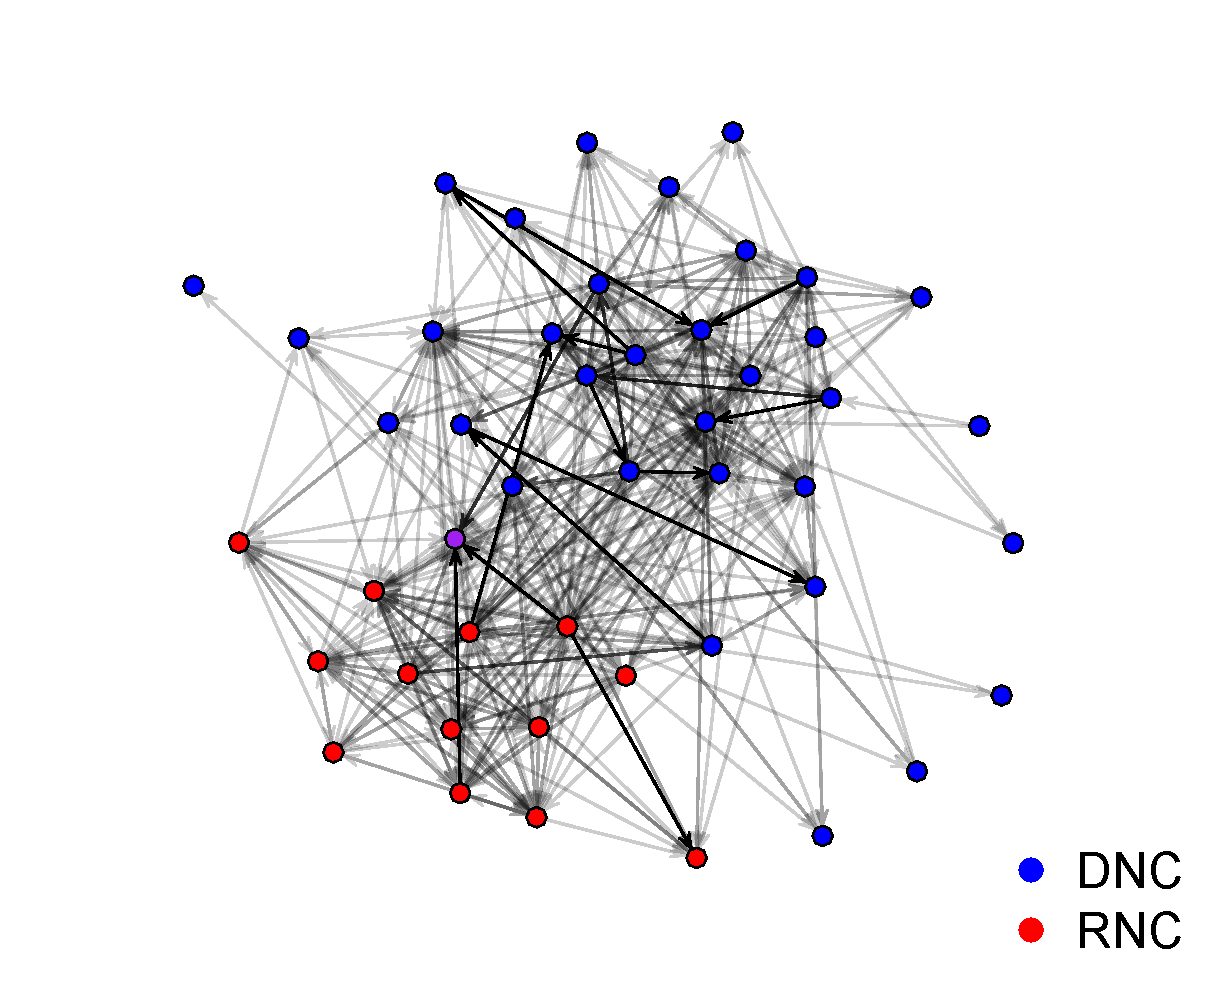
\includegraphics[width=.85\linewidth]{graphics/combinedGraph}

\end{block}

\end{columns}

\end{frame}

%%%%%%%%%%%%%%%%%%%%%%%%%%%%%%%%%
%%%% Movies
%%%%%%%%%%%%%%%%%%%%%%%%%%%%%%%%%


\begin{frame}
\begin{block}{DNC Convention}
\center
\includemovie[controls]{6cm}{6cm}{dncrnc_dnccon.swf}
\end{block}
\end{frame}

\begin{frame}
\begin{block}{RNC Convention}
\center
\includemovie[controls]{6cm}{6cm}{dncrnc_rnccon.swf}
\end{block}
\end{frame}

\begin{frame}
\begin{block}{Election Day}
\center
\includemovie[controls]{6cm}{6cm}{dncrnc_elect.swf}
\end{block}
\end{frame}



%%%%%%%%%%%%%%%%%%%%%%%%%%%%%%%%%
%%%% Movies
%%%%%%%%%%%%%%%%%%%%%%%%%%%%%%%%%

\subsection{Network Evolution as a Decision Process}


\begin{frame}
\frametitle{Network Evolution as a Decision Process}

\begin{block}{}
Those blogs credentialed during the 2004 electoral cycle represented a small ``elite'' circle of especially active authors, whose blogs centered on coverage of politics and current events.
\end{block}

\begin{columns}
\column{.5\textwidth}


\begin{block}{Model as}
\begin{itemize}
\item Dynamic decision process
\item Blog authors select those to whom they link in response to context and past history
\end{itemize}
\end{block}


\column{.5\textwidth}

\begin{block}{Actor-oriented Model}
\begin{itemize}
\item \citep{snijders96,snijders97,snijders01}
\item Employ a somewhat simpler version of this general scheme, which represents network evolution as a discrete time logistic choice process \citep{mcfadden76,mcfadden74}
\end{itemize}
\end{block}

\end{columns}


\end{frame}

\subsection{Edge Updating as Logistic Choice}

%%%%%%%%%%%%%%%%%%%%%%%%%%%%%%%%%
%%%% Slide
%%%%%%%%%%%%%%%%%%%%%%%%%%%%%%%%%

\begin{frame}
\frametitle{Network Evolution as a Decision Process}

\begin{block}{}
At its crudest level, a blog is a web page with dynamically updated links to other online resources.  
\end{block}

\begin{block}{Assumptions}
\begin{enumerate}
\item The state of outgoing edges at each observation of the blog network is assumed to result from the choices of the sending blog;
\item Each blog in the network may send an edge to any number of other blogs in the network at any time;
\item The decision of a given blog regarding the state of a given edge is made myopically, and in isolation;
\item The decision of a given blog regarding the state of a given edge may depend upon the past history of the blog network, or of the current external context.
\end{enumerate}

\end{block}


\end{frame}

\begin{frame}
\begin{block}{}
\begin{itemize}
\item \emph{utility function,} $u$
\item $A_{ij,t}=0$ and $A_{ij,t}=1$, the odds that $i$ will choose $A_{ij,t}=1$ are strictly increasing in $u_i(A|A_{ij,t}=1)/u_i(A|A_{ij,t}=0)$
\item \emph{stochastic choice} process
\item We employ a  \emph{logistic choice} model
\end{itemize}
\end{block}
\begin{block}{}
\begin{equation}
\Pr(A_{ij,t}=1) = \frac{\exp\left[u_i\left(A|A_{ij,t}=1\right)\right]}{\exp\left[u_i\left(A|A_{ij,t}=1\right)\right]+\exp\left[u_i\left(A|A_{ij,t}=0\right)\right]}, \label{eq:logit1}
\end{equation}
or, equivalently, that
\begin{equation}
\textrm{logit}(A_{ij,t}) = \ln\frac{\Pr(A_{ij,t}=1)}{\Pr(A_{ij,t}=0)} = u_i\left(A|A_{ij,t}=1\right)-u_i\left(A|A_{ij,t}=0\right),\label{eq:logit2}
\end{equation}
\end{block}

\end{frame}

%%%%%%%%%%%%%%%%%%%%%%%%%%%%%%%%%
%%%% Slide
%%%%%%%%%%%%%%%%%%%%%%%%%%%%%%%%%

\section{Potential Payoff Elements: The Hypotheses}

\begin{frame}
\frametitle{Mixing}

\begin{block}{}
\begin{description}
\item[Mixing Hypothesis 1] The partial payoff of an edge from blog $i$ to blog $j$ will be lower if $i$ and $j$ do not belong to the same credentialing faction than if $i$ and $j$ belong to the same faction.
\item[Mixing Hypothesis 2] The partial payoff of an edge from blog $i$ to blog $j$ will be the same or higher if $i$ and $j$ do not belong to the same credentialing faction than if $i$ and $j$ belong to the same faction.
\end{description}
\end{block}

\end{frame}


\begin{frame}
\frametitle{Balance-Theoretic Influences}

\begin{block}{}
\begin{description}
\item[BT Hypothesis 1: ``Friend of a friend'' (In-Group two paths)] We hypothesize that the partial payoff for a link from blog $i$ to blog $j$ is increasing in the number of $i,j$ two-paths contained in the same faction, (for ex. in this case, the RNC or DNC).  In other words, the payoff for Ego to form a relationship with a ``friendly" is enhanced if that friendly is also connected to Ego via another ``friendly".


\item[BT Hypothesis 2: ``Friend of an enemy'' (Cross-Group two paths)] We hypothesize that the partial payoff for a link from blog $i$ to blog $j$ is decreasing in the number of two paths through individuals of the same faction as $i$, where $j$ and $i$ belong to different factions. 

\end{description}

\end{block}

\end{frame}

\begin{frame}
\frametitle{Balance-Theoretic Influences}

\begin{block}{}
\begin{description}

\item[BT Hypothesis 3: Reciprocity (``friendly'')]  We hypothesize that reciprocity will be accompanied with positive gains for ingroup edge creation and low or negative gains for across-group citation. In this case citations are primarily a positive relation such that utility gain comes from increasing the prominence of ones friends and not through competition with ones enemies. 

\item[BT Hypothesis 4: Reciprocity (``hostile'')]  Conversely we hypothesize that reciprocity will be accompanied with positive gains for outgroup edge creation and low or negative gains for ingroup citation. In this case citations are primarily a negative relation such that utility gain comes from refuting enemies' accusations. 
\end{description}

\end{block}

\end{frame}

\begin{frame}
\frametitle{Context and Seasonality}

\begin{block}{}
\begin{description}

\item[Seasonality Hypothesis 1]\cite{butts09} found that the volatility of the blog networks changes with time of day, day of week, and period in the electoral cycle.  One way in which ``volatility'' might manifest in this case is through an increase or decrease degree of inertia in the network structure.  Thus, the partial payoff to continuing a previous action is predicted to follow seasonal and periodic patterns.

\item[Seasonality Hypothesis 2] We suspect that overall propensity to send links will vary over time. We argue that ego's linking to others involves a search process, and is consumptive of attentional/energetic resources. Resource availability varies seasonally, and with it the partial payoff for sending links per se.

\end{description}

\end{block}
\end{frame}

\begin{frame}
\frametitle{Context and Seasonality}

\begin{block}{}
\begin{description}

\item[Seasonality Hypothesis 3] We propose that behavioral factors might change with time and context: 

\emph{Selective salience} --  We might expect that there would be larger propensity to create ties across or within group during important events in the election cycle.

\end{description}

\end{block}

\end{frame}

\section{Methods}

\subsection{Inferential Framework}

\begin{frame}

\begin{block}{
\center
Inferential Framework\\

\

}
\end{block}
\end{frame}


\begin{frame}
\frametitle{Dynamic Lagged-Logistic Network Regression}

\begin{block}{}
This work employs the methodology -- Dynamic Lagged-Logistic Regression -- recommended by \cite{almquist10} for large dynamic data-sets, which builds on the Exponential Random Graph \citep{holland81a, holland81b, butts08, snijders06,strauss} and Logistic Network Regression literatures \citep{krackhardt87a,krackhardt87b,krackhardt88}.
\end{block}

\begin{block}{}
 \begin{align}
\textrm{logit}(A_{ij,t}) = \theta^t\left[t_{ij}(A|A_{ij,t}=1,X)-t_{ij}(A|A_{ij,t}=0,X)\right]
\end{align}
\end{block}

\end{frame}


\section{Analysis and Results}

\begin{frame}
\frametitle{Analysis: GOF}

\begin{block}{}
\includegraphics[width=1\linewidth]{graphics/gof100}
\end{block}
\end{frame}


\begin{frame}
\frametitle{Results}

\input models.tex

\end{frame}

\begin{frame}
\frametitle{Results}

\input models1.tex

\end{frame}

\section{Discusion and Findings}

\begin{frame}
\frametitle{Results}

\begin{block}{Heiderian}

\begin{itemize}
\item Accept BT hypothesis 1 --  Reject BT hypothesis 2.

\item Between-group reciprocity is increased and in-group reciprocity decreases the likelihood of creating a tie

\begin{itemize}
\item Suggesting blog warring
\end{itemize}

\end{itemize}

\end{block}

\begin{columns}
\column{.4\textwidth}


\begin{block}{RNC vs DNC}
\begin{itemize}
\item Larger propensity to link within-group
\item Larger propensity to link between-group 
\end{itemize}
\end{block}


\column{.6\textwidth}

\begin{block}{Temporal and Period Effects}
\begin{itemize}
\item 
\item Strong inertial-- Accept SH 2
\item Period: Decrease in activity during election (otherwise stable) -- Reject SH 3
\end{itemize}
\end{block}

\end{columns}


\end{frame}




%%%%%%%%%%%%%%%%%%%%%%%%%%%%%%%%%
%%%% Thank You
%%%%%%%%%%%%%%%%%%%%%%%%%%%%%%%%%
\begin{frame}
\begin{block}{}
\begin{center}
Thank You!
\end{center}
\end{block}
\end{frame}
%%%%%%%%%%%%%%%%%%%%%%%%%%%%%%%%%
%%%% Thank You
%%%%%%%%%%%%%%%%%%%%%%%%%%%%%%%%%

%%%%%%%%%%%%%%%%%%%%%%%%%%%%%%%%%
%%%% References
%%%%%%%%%%%%%%%%%%%%%%%%%%%%%%%%%
\begin{frame}[allowframebreaks] 
\frametitle{References}
\def\newblock{}
\bibliographystyle{ajs}
\bibliography{netsandorgs}
\end{frame}
%%%%%%%%%%%%%%%%%%%%%%%%%%%%%%%%%
%%%% References
%%%%%%%%%%%%%%%%%%%%%%%%%%%%%%%%%



















\end{document}

